\documentclass[11pt]{beamer}

\usetheme{metropolis}

\usepackage{graphicx}
\usepackage{physics}
\usepackage{adjustbox}
\usepackage{caption}
\usepackage{chemformula}
\usepackage{quoting}
\usepackage[style=chem-angew,backend=bibtex]{biblatex}
\bibliography{references}
%
% Choose how your presentation looks.
%
% For more themes, color themes and font themes, see:
% http://deic.uab.es/~iblanes/beamer_gallery/index_by_theme.html
%
\mode<presentation>
{
  \usetheme{default}      % or try Darmstadt, Madrid, Warsaw, ...
  \usecolortheme{default} % or try albatross, beaver, crane, ...
  \usefonttheme{default}  % or try serif, structurebold, ...
  \setbeamertemplate{navigation symbols}{}
  \setbeamertemplate{caption}[numbered]
  \setbeamerfont{footnote}{size=\tiny}
} 

\usepackage[english]{babel}
\usepackage[utf8]{inputenc}
\graphicspath{{../lectureMW/image/}}

\AtBeginSection[]{
\begin{frame}{Outline}
  \tableofcontents[currentsection]
\end{frame}
}

\title{Chapter 7: Electronic Structure of the Atom}
\institute{Chemistry Department, Cypress College}
\date{October 13, 2022}

\begin{document}

\begin{frame}
  \titlepage
\end{frame}

\begin{frame}{Class Announcements}
  \textbf{Lecture}
  \begin{itemize}
  \item Go over homework 6 (EC for students who present)
  \item Finish up Ch 6 and worksheets 7 and 8; begin discussion on Ch 7
    - Electronic Structure of the Atom
  \item Quiz and Homework assignment released Fri, Oct 21th at 3pm
  \item Exam 2 details and exam review session
  \end{itemize}
\end{frame}

\section{Review: Energy Changes}

\begin{frame}{Law of Conservation of Energy}
  \begin{center}
    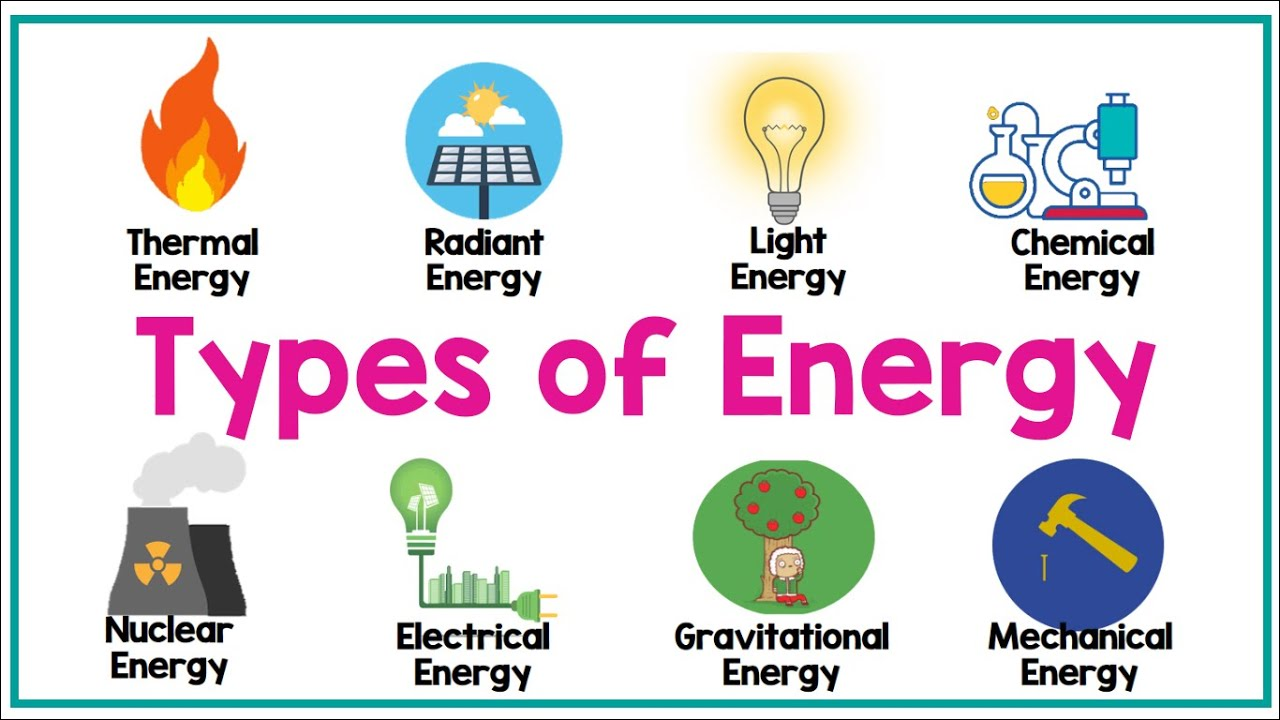
\includegraphics[scale=0.13]{energy_types}
    
    \textbf{Energy is neither created nor destroyed}
  \end{center}

  \begin{itemize}
  \item Energy can be converted from form to another
    e.g. mechanical, chemical, thermal, nuclear,
    electrical and vibrational energy
  \item Converting from one energy form to another is
    never $100\%$ efficient; there is always a loss of
    energy measured in Joules (J)
  \end{itemize}
\end{frame}

\begin{frame}{Endothermic Reaction Diagram}
  \centering
  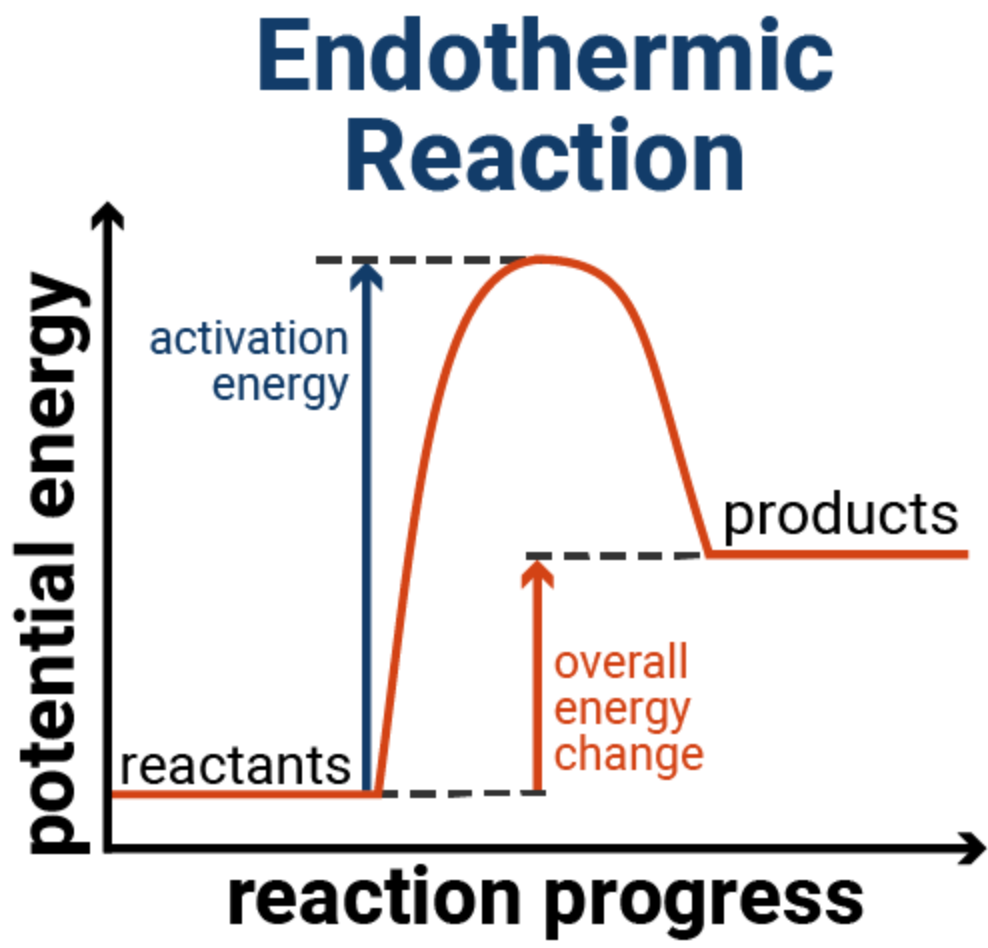
\includegraphics[width=0.5\linewidth]{endo_rxn}

  \begin{itemize}
  \item \textbf{Recall Potential energy} - ability to do
    work; $\Delta E_\text{products} > \Delta E_\text{reactants}$
  \item \textbf{Activation energy} - minimum energy to start the
    reaction; determines the rate at which the reaction undergoes
  \end{itemize}
\end{frame}

\begin{frame}{Exothermic Reaction Diagram}
  \centering
  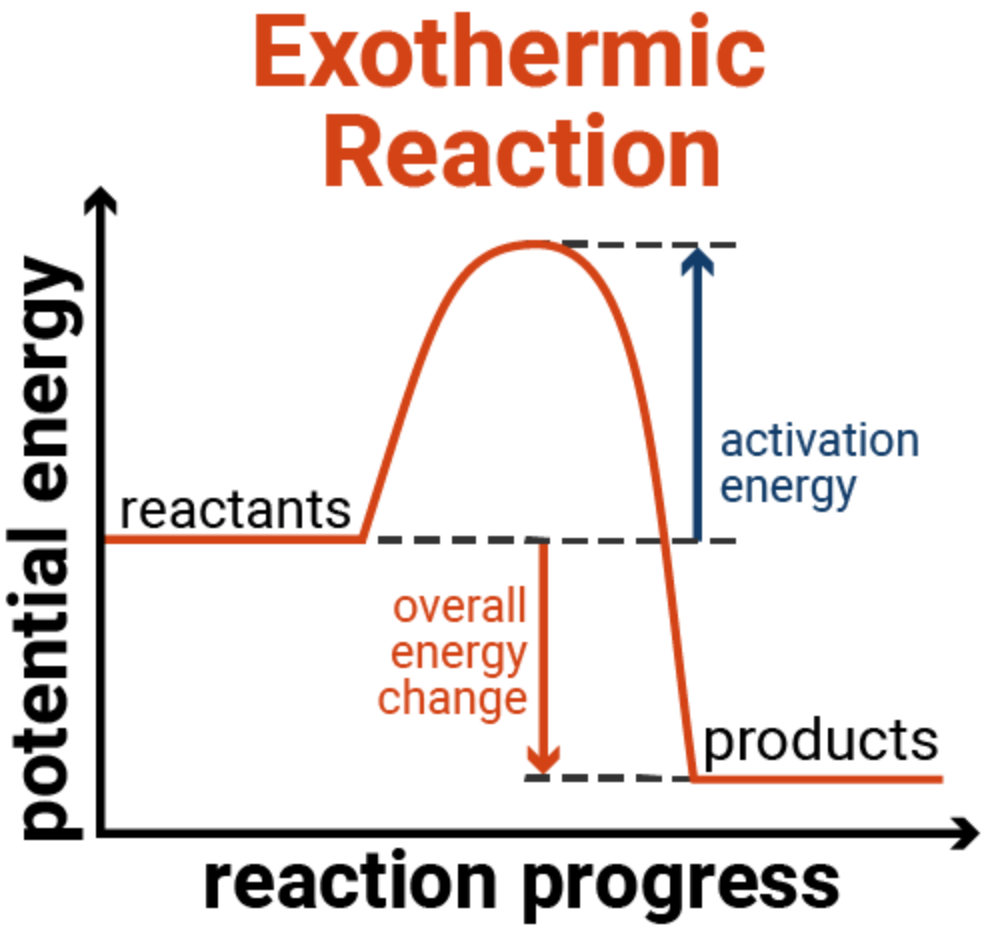
\includegraphics[width=0.5\linewidth]{exo_rxn}
  \begin{itemize}
  \item \textbf{Potential energy} - $\Delta E_\text{products} < \Delta E_\text{reactants}$
  \item Products are more stable than reactants since preference
    for lower energy state
  \end{itemize}
\end{frame}

\begin{frame}{Calorimetry}
  \begin{columns}
    \column{0.3\textwidth}
    \begin{center}
      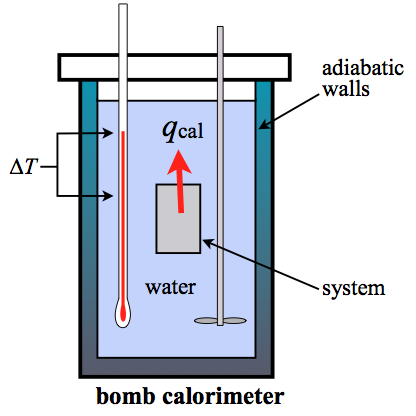
\includegraphics[scale=0.3]{bomb_calor}
    \end{center}
    \column{0.55\textwidth}
    \begin{equation}
      q = mC\Delta T
    \end{equation}
    where $q$ is heat, $m$ is the mass (g), $C$ is
    specific heat capacity (J/($^\circ$C g)) and $T$ is
    temperature ($^\circ$C)
  \end{columns}
  
  \begin{itemize}
  \item Performed at constant-pressure (atomospheric pressure)
  \item Bomb Calorimeter is Insulated where the heat evolved by the reaction
    is absorbed by the water
  \item \textbf{Specific Heat Capacity} - the amount of heat ($q$)
    required to heat an object 1$^\circ$C/g
  \end{itemize}
\end{frame}

\begin{frame}{Relating Conservation of Energy}
  \centering
  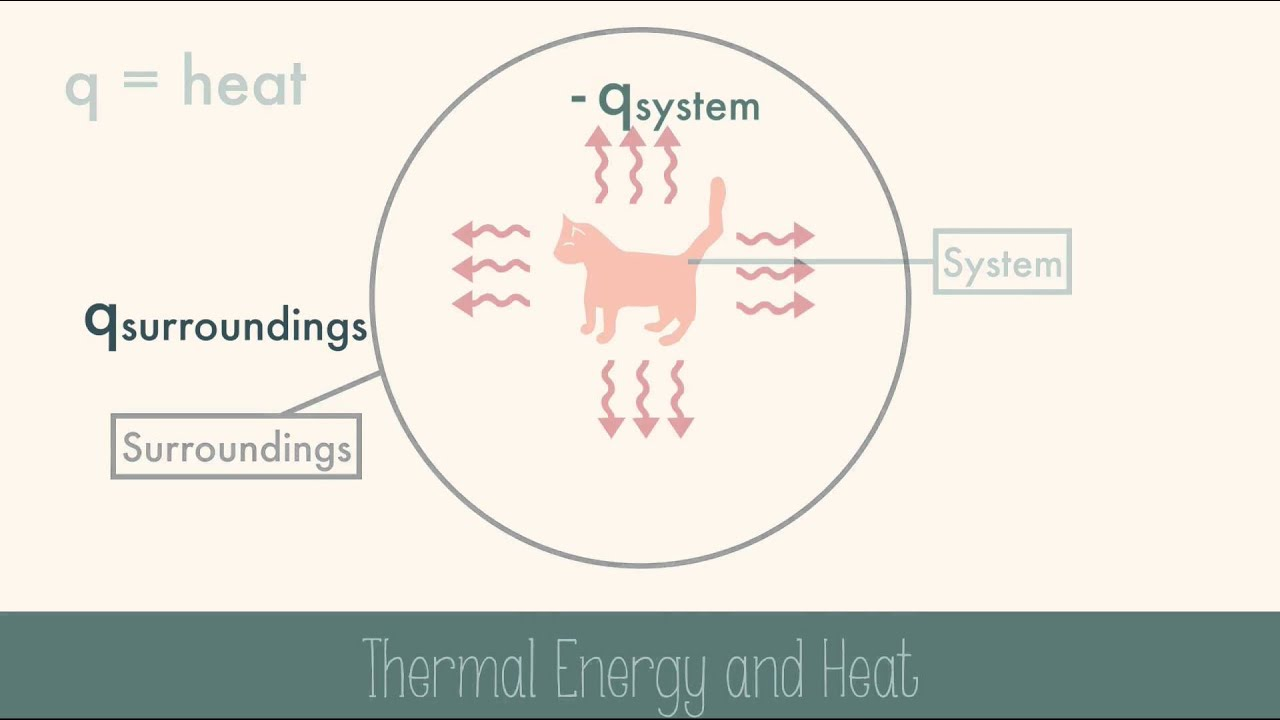
\includegraphics[width=0.8\textwidth]{heat_sys}

  $q_\text{system} + q_\text{surrounding} = 0$
  where $q$ is the heat

  Negative sign indicate released heat and positive sign indicates
  absorbed heat
\end{frame}

\section{Electromagnetic Radiation and Energy}

\begin{frame}{Electromagnetic Radiation}
  \centering
  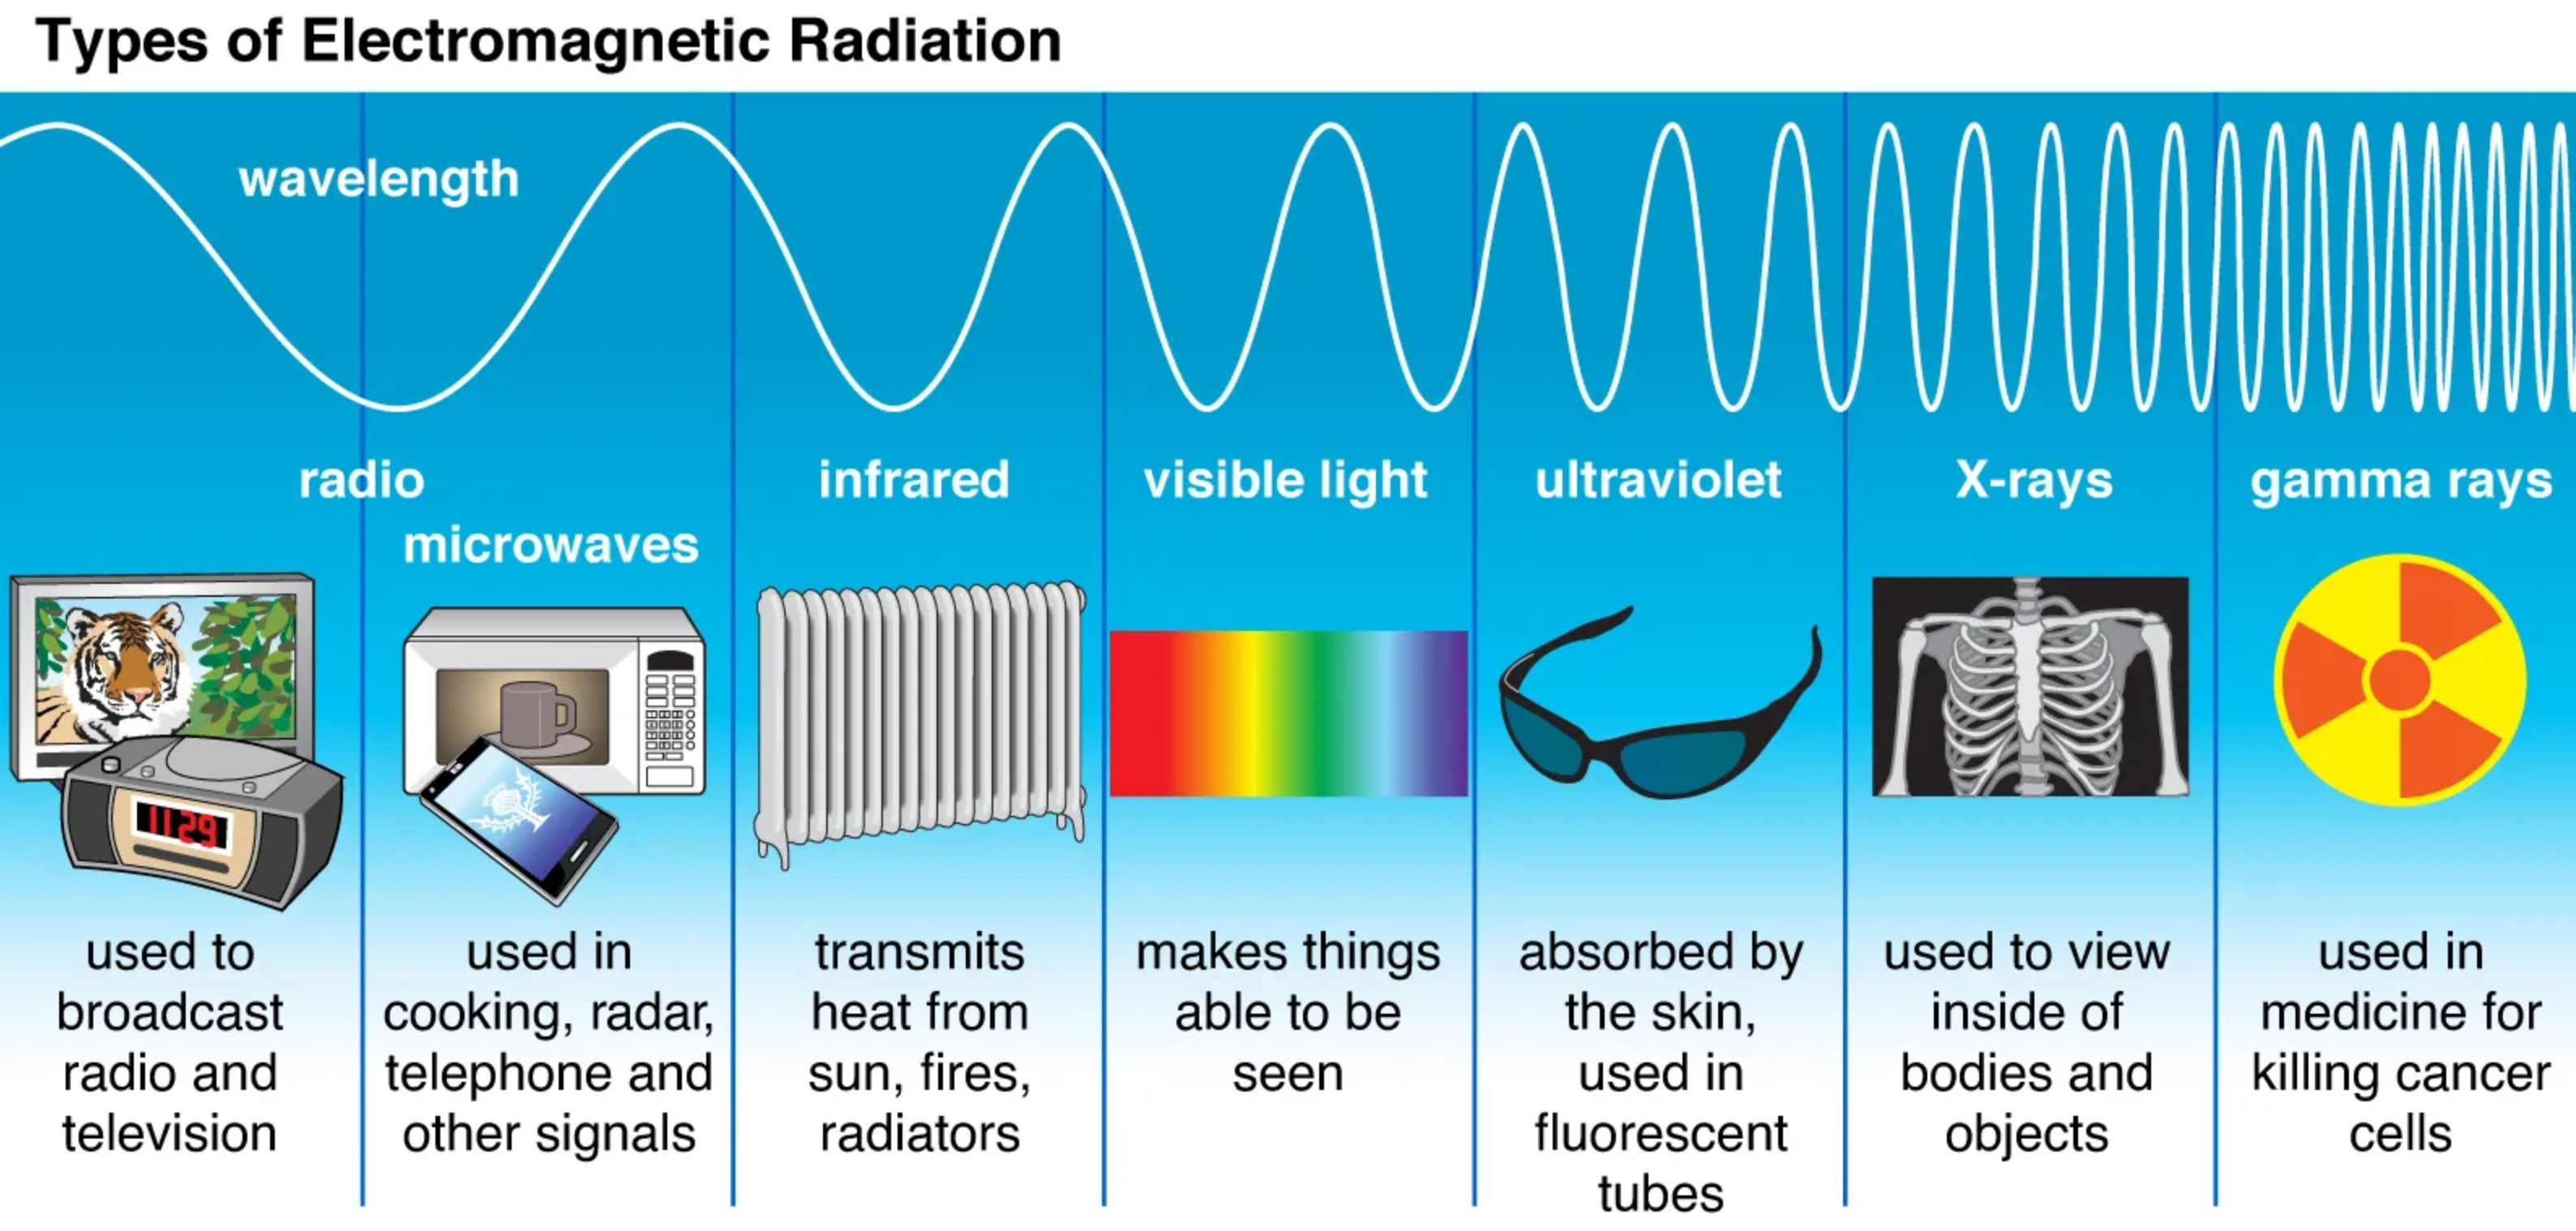
\includegraphics[width=0.8\linewidth]{electromag_types}

  \begin{itemize}
  \item Different types of radiation that are a form of energy
  \begin{equation}
    E = \frac{hc}{\lambda} = h\nu
  \end{equation}
  \item[] where $\lambda$ is the wavelength (m), $c$ is the speed
    of light ($3.00 \times 10^8$ m/s), $h$ is the Planck constant
    ($6.626 \times 10^{-34}$ J s) and $E$ is energy (J)
  \end{itemize}
\end{frame}

\begin{frame}{Electromagnetic Radiation}
  \begin{center}
  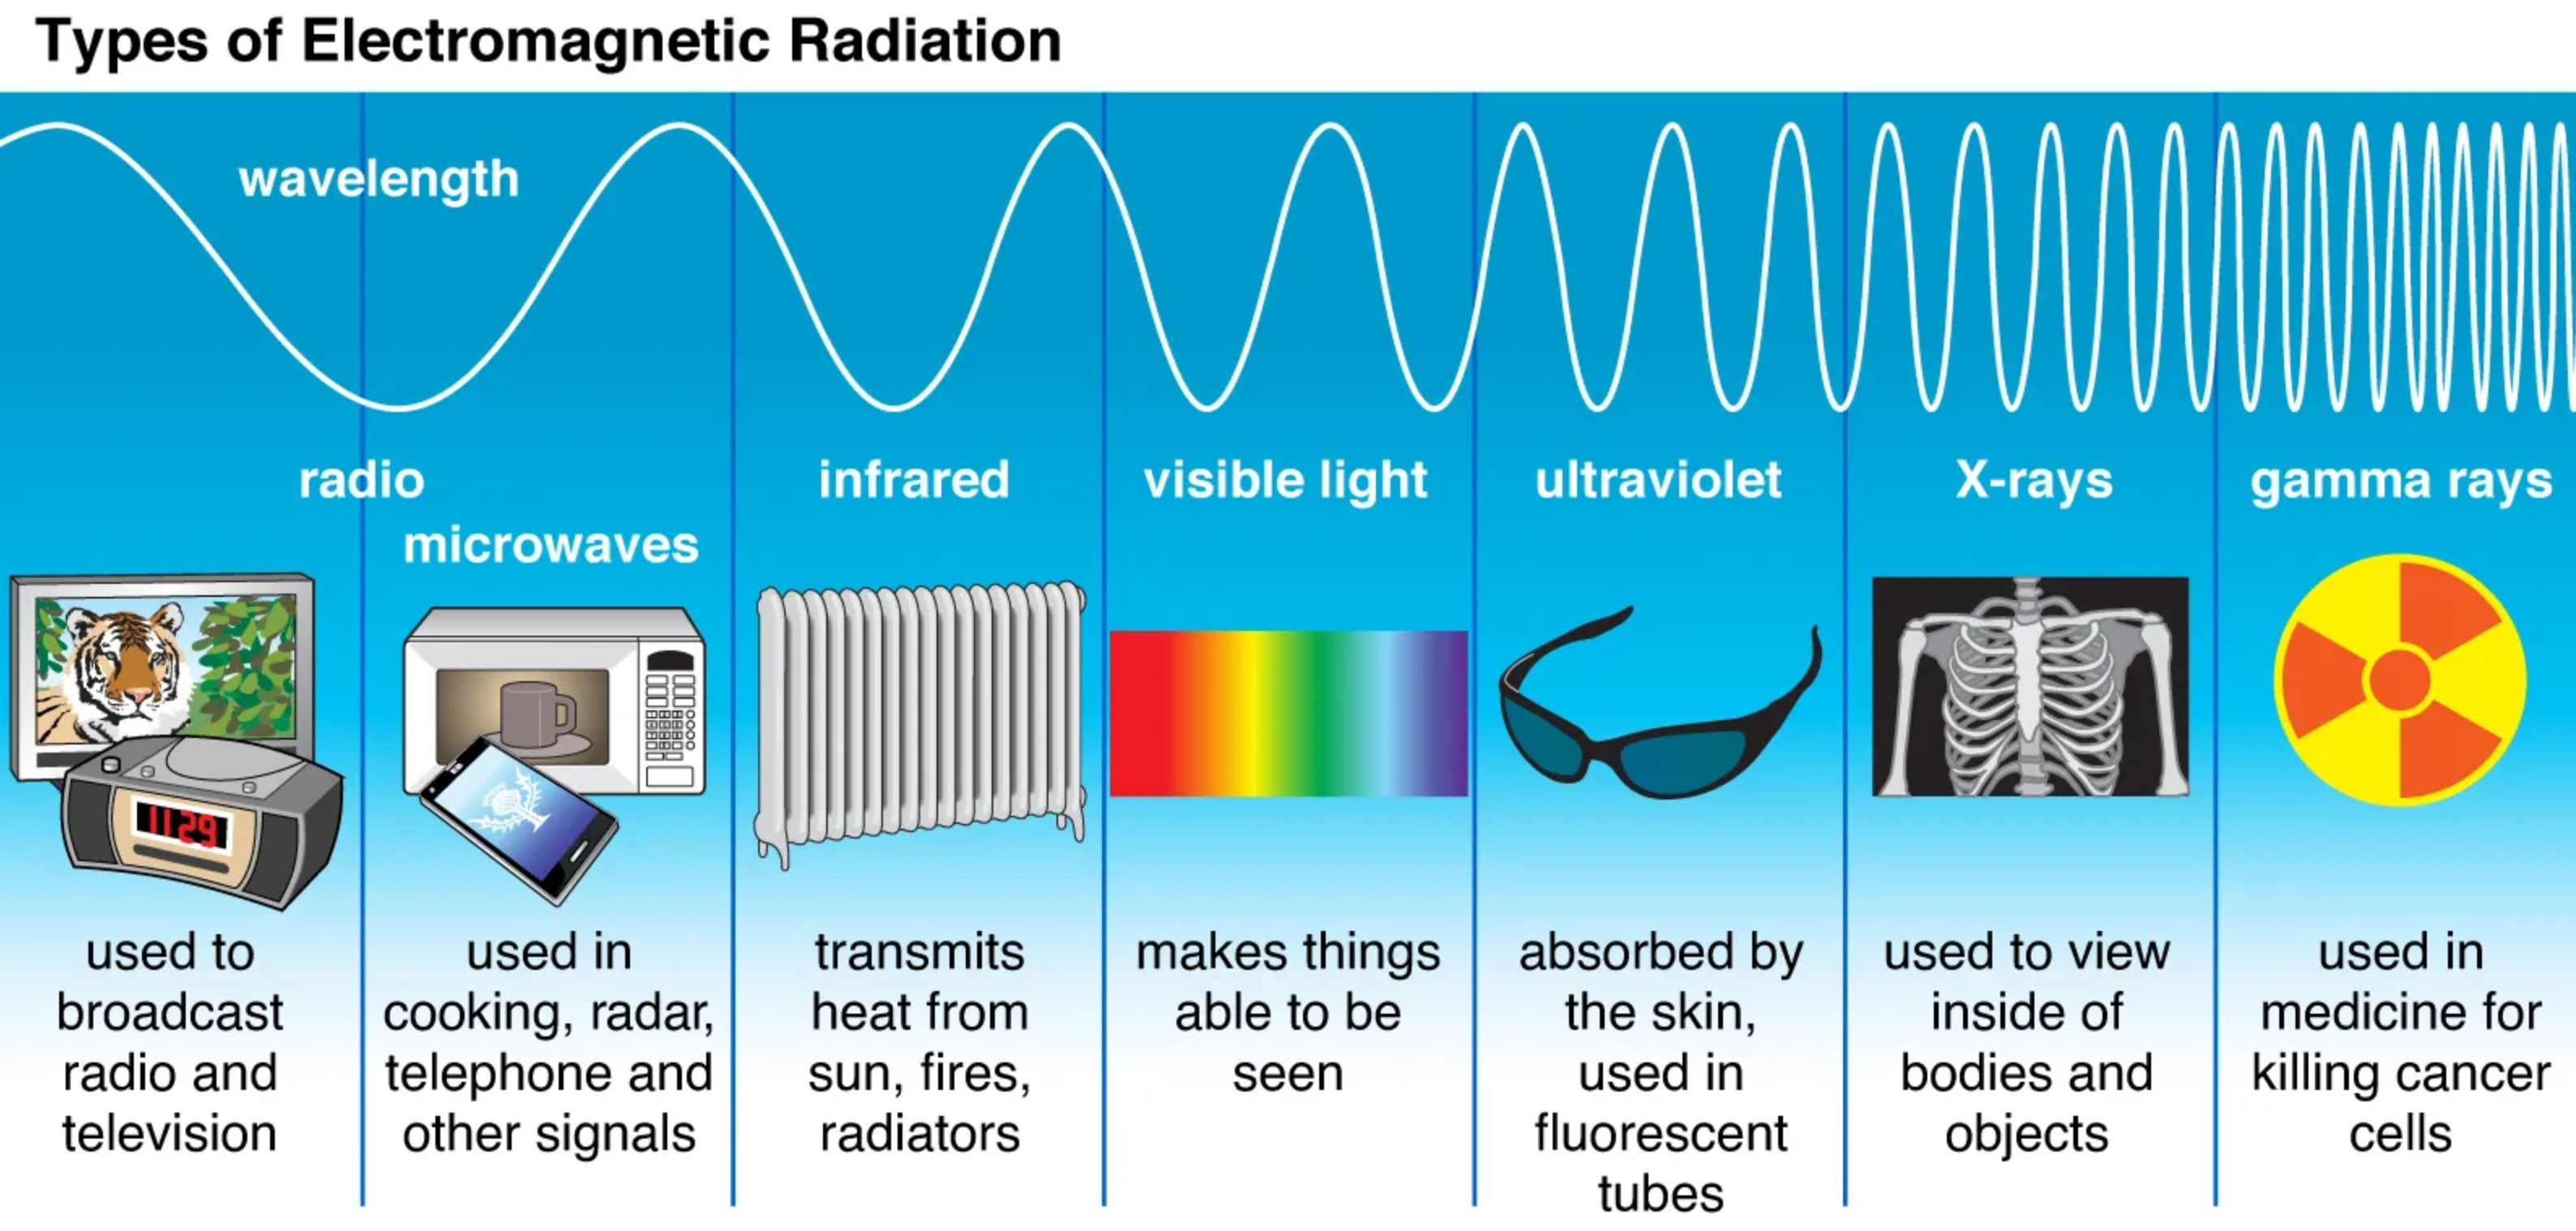
\includegraphics[width=0.8\linewidth]{electromag_types}
  \end{center}
  Relationship of speed of light ($c$) to frequency in 1/s or Hz ($\nu$) and
  wavelength in m ($\lambda$)
  \begin{equation}
    c = \nu\lambda
  \end{equation}
  Speed of light is $3.00\times 10^8$ m/s
\end{frame}

\begin{frame}{What is a wavelength and frequency?}
  \centering
  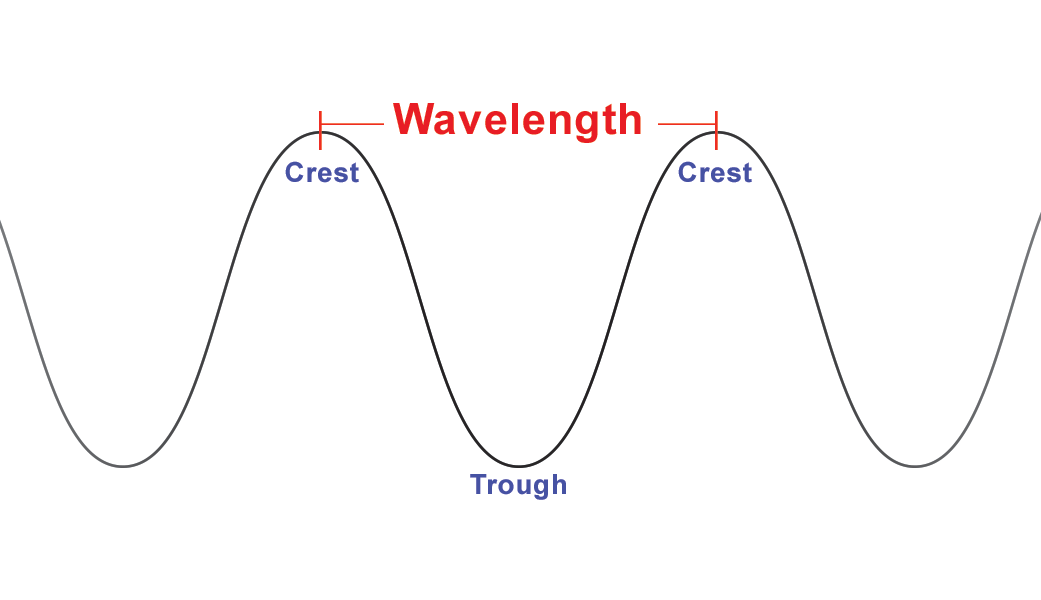
\includegraphics[width=0.8\linewidth]{wavelength}
\end{frame}

\begin{frame}{Relating to Visible Light}
  \centering
  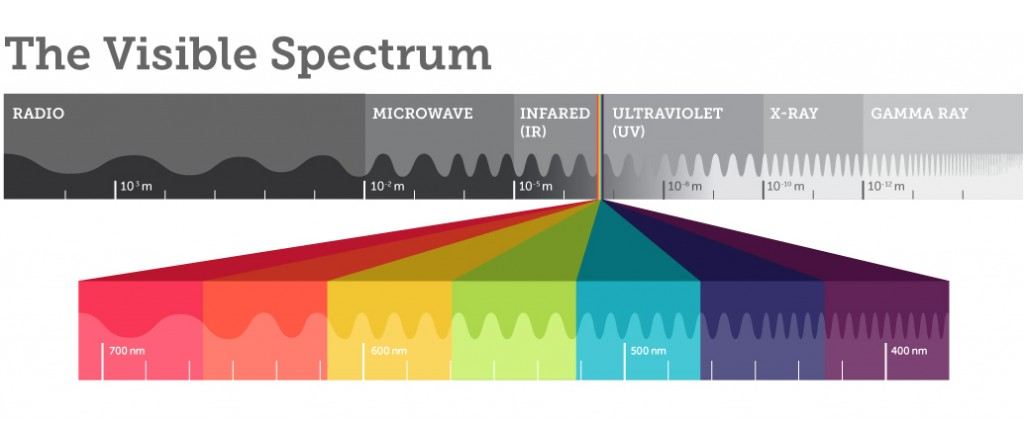
\includegraphics[width=0.85\linewidth]{visible_light}
  
  Visible light range from 700nm to 400nm;
  ROYGBV
  
  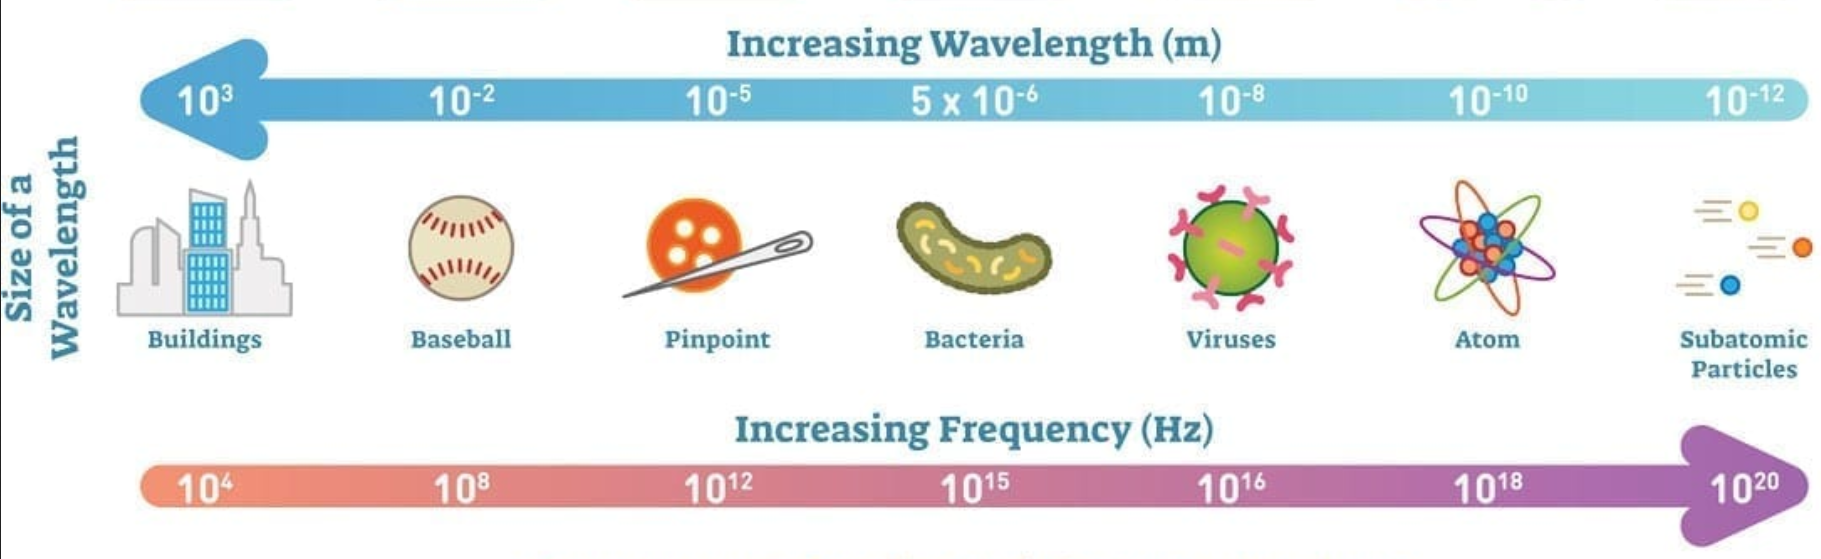
\includegraphics[width=0.85\linewidth]{wave_freq_size}
\end{frame}

\begin{frame}{Revisit: Radiation Energy}
  \begin{center}
    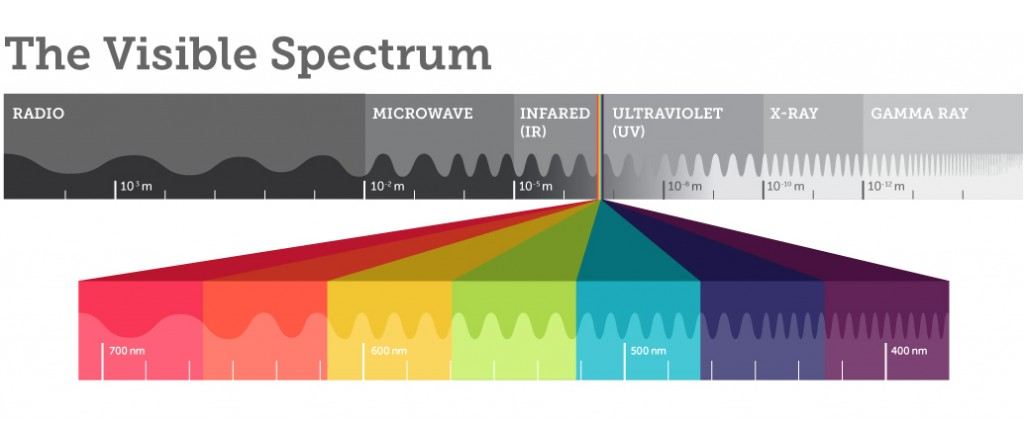
\includegraphics[width=0.85\linewidth]{visible_light}
  \end{center}
  \begin{equation}
    E = \frac{hc}{\lambda} = h\nu
    \label{eqn:photon}
  \end{equation}
  \begin{itemize}
  \item High frequency and larger wavelengths lead to higher radiation
    energy
  \item Energy are contained in packages known as photons; Eqn \ref{eqn:photon}
    computes the energy for 1 photon
  \end{itemize}
\end{frame}

\begin{frame}{Practice: Sunlight Energy}
  The sun emits a wide range of electromagnetic radiation including
  visible, infrared, and ultraviolet light.

  a) Which type of light has the longest wavelength: visible, infrared,
  or ultraviolet?

  b) Which has the highest frequency?

  c) Which is composed of the highest-energy photons
  \vfill
\end{frame}

\begin{frame}{Example: Calculating $\lambda$, $\nu$, and $E$}
  Infrared light emitted from a TV remote control or from a wireless
  computer mouse has a wavelength of 805nm.

  a) What is the frequency of the light?

  b) What is the energy of its photons?

  \onslide<2->{\textbf{a)}
    \begin{align*}
      \nu\lambda = & c \\
      \nu = & \frac{c}{\lambda} = \frac{3.00\times 10^8\text{m/s}}{8.05\times 10^{-7}\text{m}}
      = 3.73 \times 10^{14}\text{Hz} 
    \end{align*}
  }
  \onslide<3->{\textbf{b)}
    \begin{align*}
      E = & h\nu = 6.626\times 10^{-34}\text{J s}\times 3.73\times 10^{14}\text{Hz} \\
      =& 2.47\times 10^{-19}\text{J}
    \end{align*}
  }
\end{frame}

\begin{frame}{Practice: TV Remote}
  If a 60-mW TV remote emits a total energy of light of $6.0\times 10^4$ J/s with
  photon energy of $2.47\times 10^{-19}$ J/photon, what is the best estimate of the
  number of photons emitted from the TV remote in 1 second: 100 photons and
  $10^{23}$ photons.
  \vfill
\end{frame}

\begin{frame}{Atomic Spectra}
  \centering
  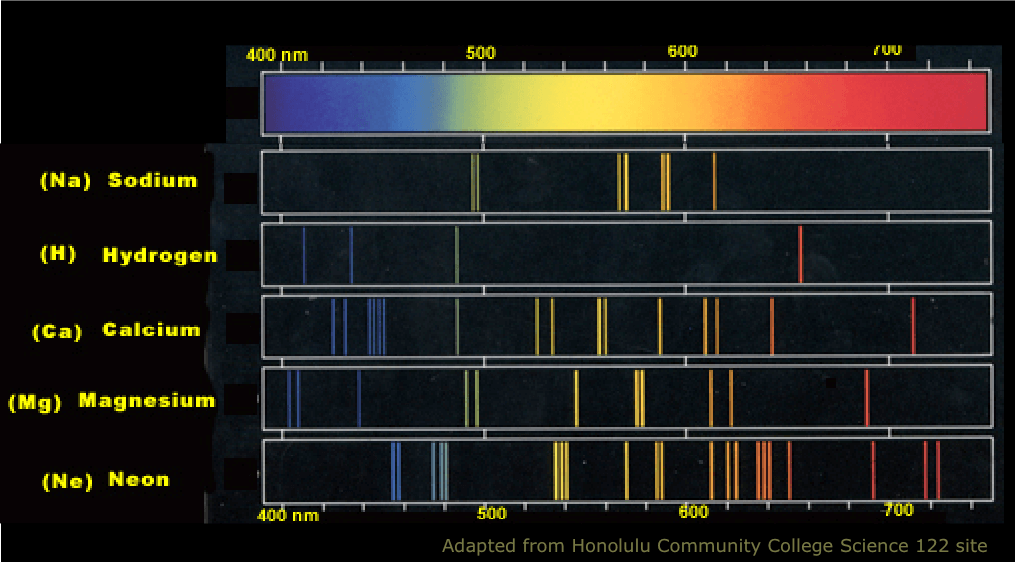
\includegraphics[width=0.85\linewidth]{cont_line}
  \begin{itemize}
  \item Continuous spectra is given at the top and
    discrete lines are emitted by atoms
  \item \textbf{Q:} Why are there discrete lines for
    the atomic spectra?
  \end{itemize}
\end{frame}

\section{Bohr Model of the H Atom}

\begin{frame}{Bohr Model}
  \begin{itemize}
  \item Energy is quantized
  \item Electrons orbit the nucleus in orbits that have
    a set size and energy
  \item The energy of the orbit is related to its size; the
    lowest energy is found in the smallest orbit
  \item Radiation is absorbed or emitted when an electron
    moves from one orbit to another
  \end{itemize}
\end{frame}

\begin{frame}{Bohr Model of the H Atom}
  \centering
  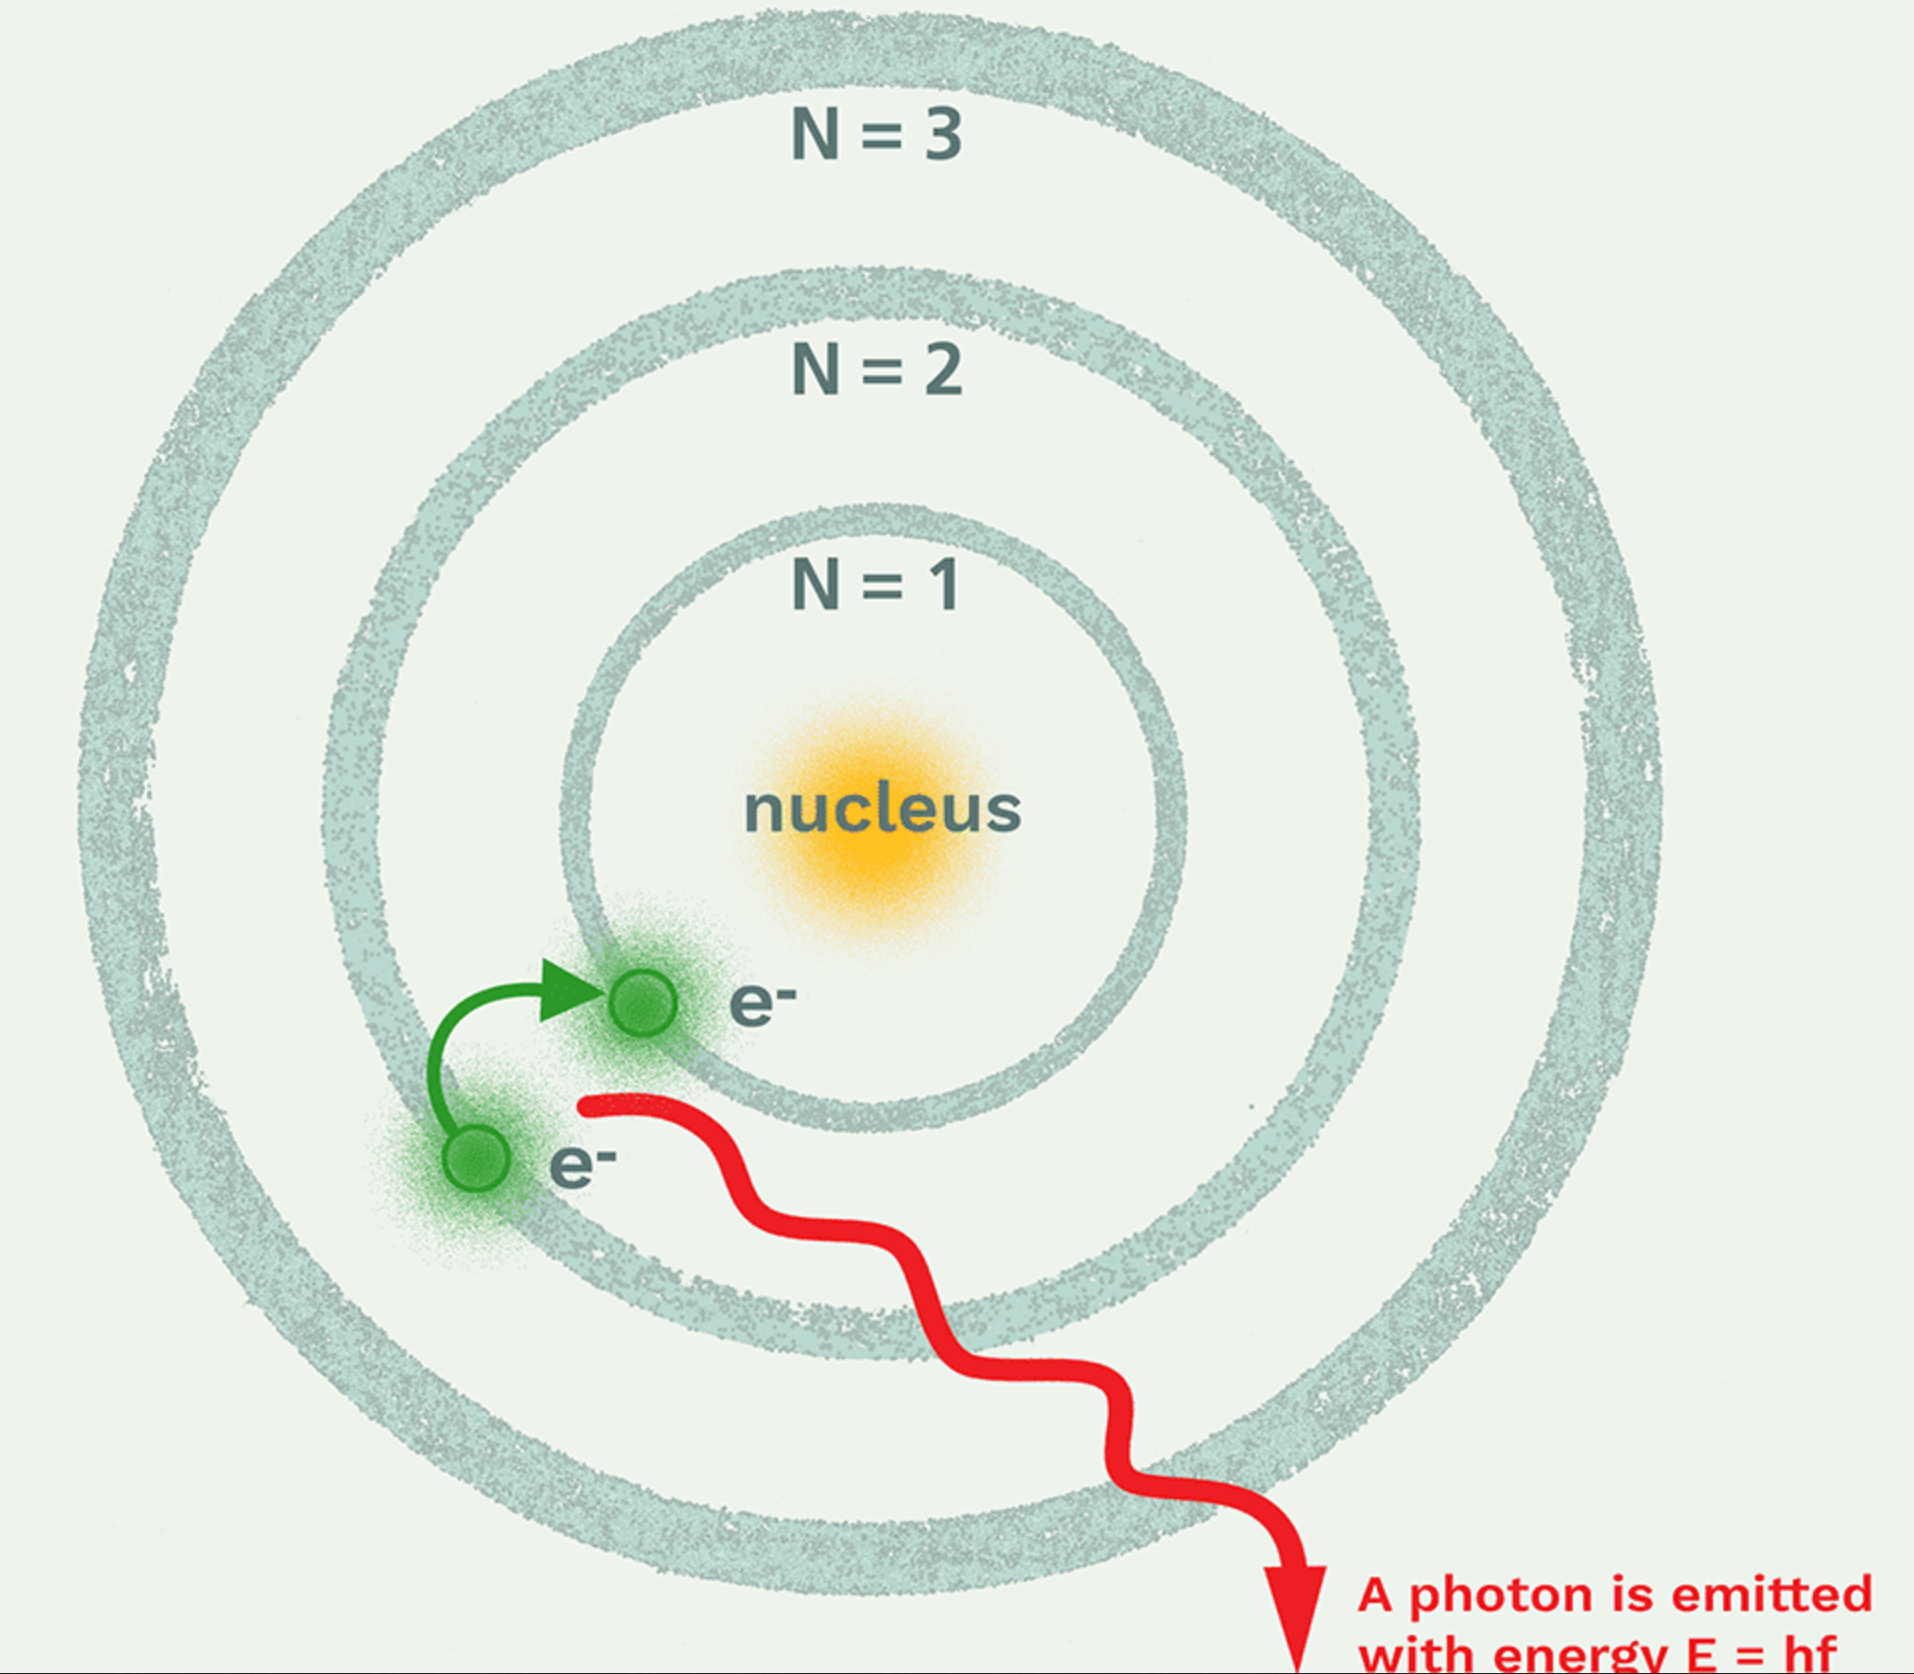
\includegraphics[width=0.55\linewidth]{bohr_model}
  \begin{align}
    \Delta E = & E_\text{final} - E_\text{initial}
  \end{align}
  Note: Keep in mind of sign conventions ($\Delta E > 0$ and
  $\Delta E < 0$)
\end{frame}

\begin{frame}{Limitation of the Bohr Model}
  \begin{itemize}
  \item Violates the Heisenberg Uncertainty Principle
  \item Poor predictions regarding the spectra of larger
    atoms
  \item Does not predict the relative intensities of spectral
    lines
  \end{itemize}
\end{frame}

\begin{frame}{Example: H atom spectra}
  Use the Bohr model of the hydrogen atom and the hydrogen
  line spectrum to answer the following. What is the photon energy
  that produces the transition between $n=2$ and $n=4$? Which transition
  from the figure has the highest transition energy?
  \begin{center}
    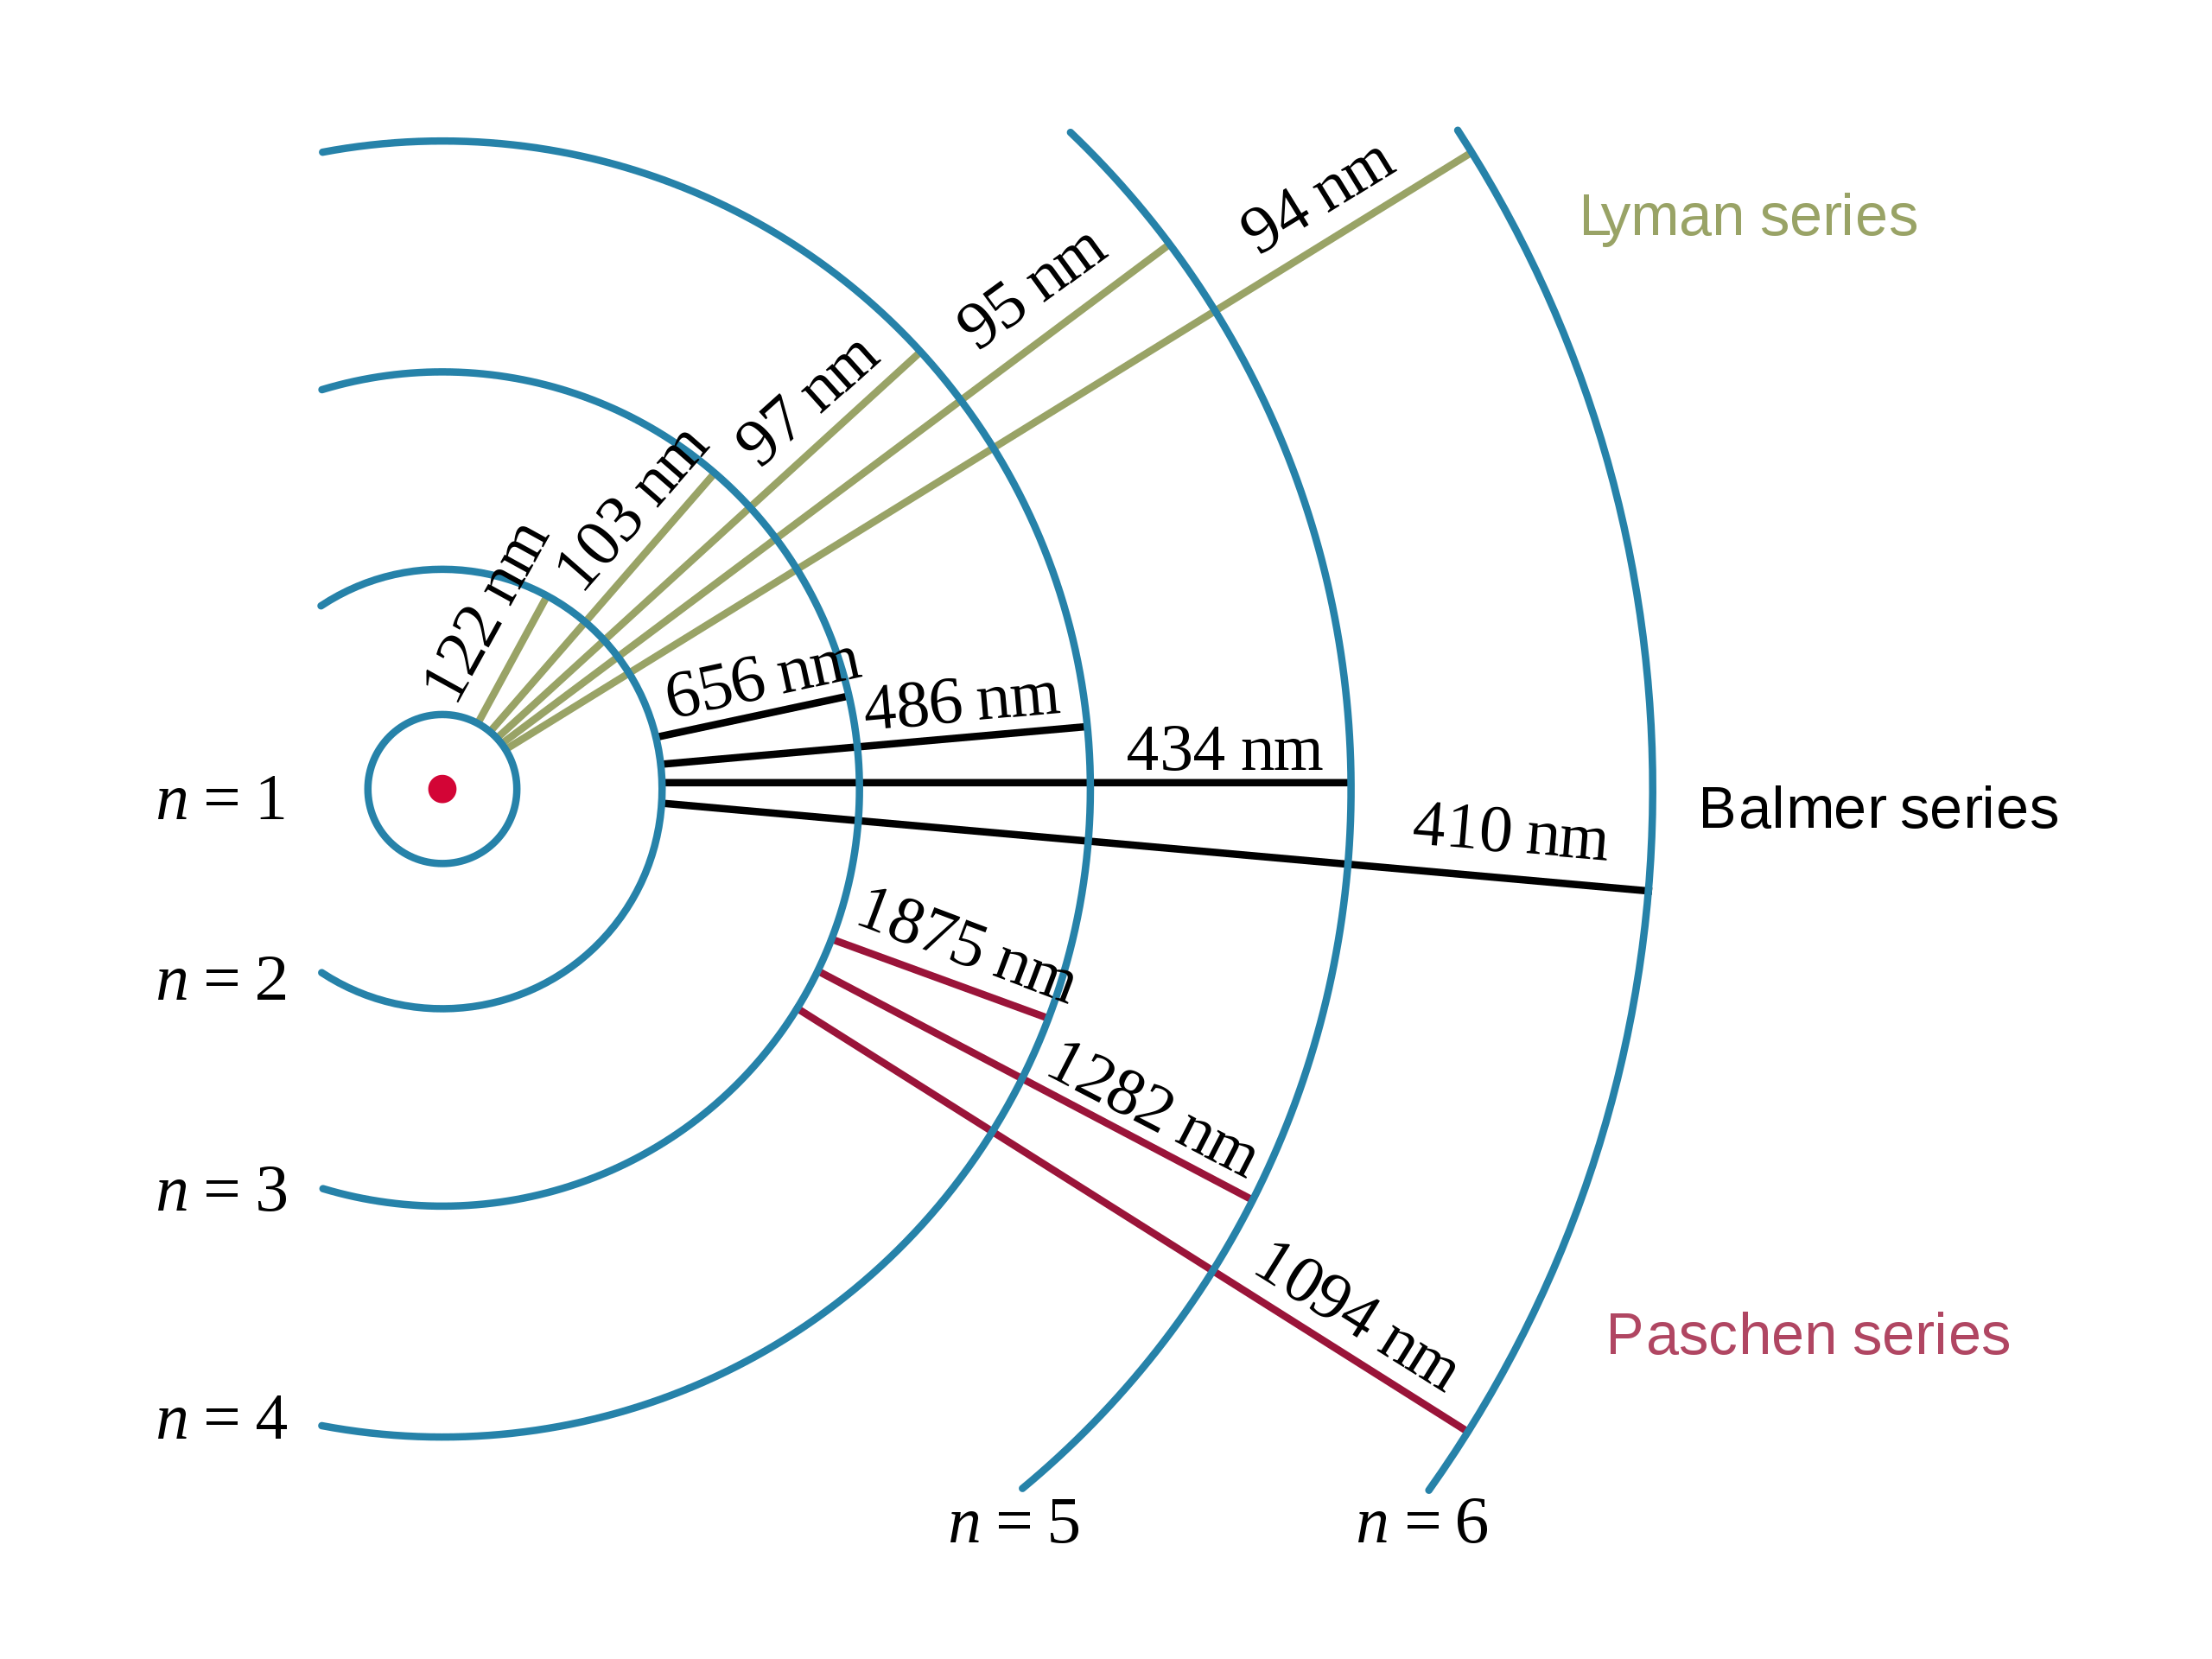
\includegraphics[scale=0.08]{h_spectra}
  \end{center}
\end{frame}

\begin{frame}{Rydberg Formula: Computing Transition $\Delta E$}
  \begin{equation}
    \frac{1}{\lambda} = -R_H\Bigg(\frac{1}{n_2^2} - \frac{1}{n_1^2}\Bigg)
  \end{equation}
  where $\lambda$ is the wavelength, $R_H$ is Rydberg constant
  ($1.09\times 10^7$ m$^{-1}$) and $n$ is the orbit state

  Note: Only applicable to hydrogen-like atoms
  \begin{center}
    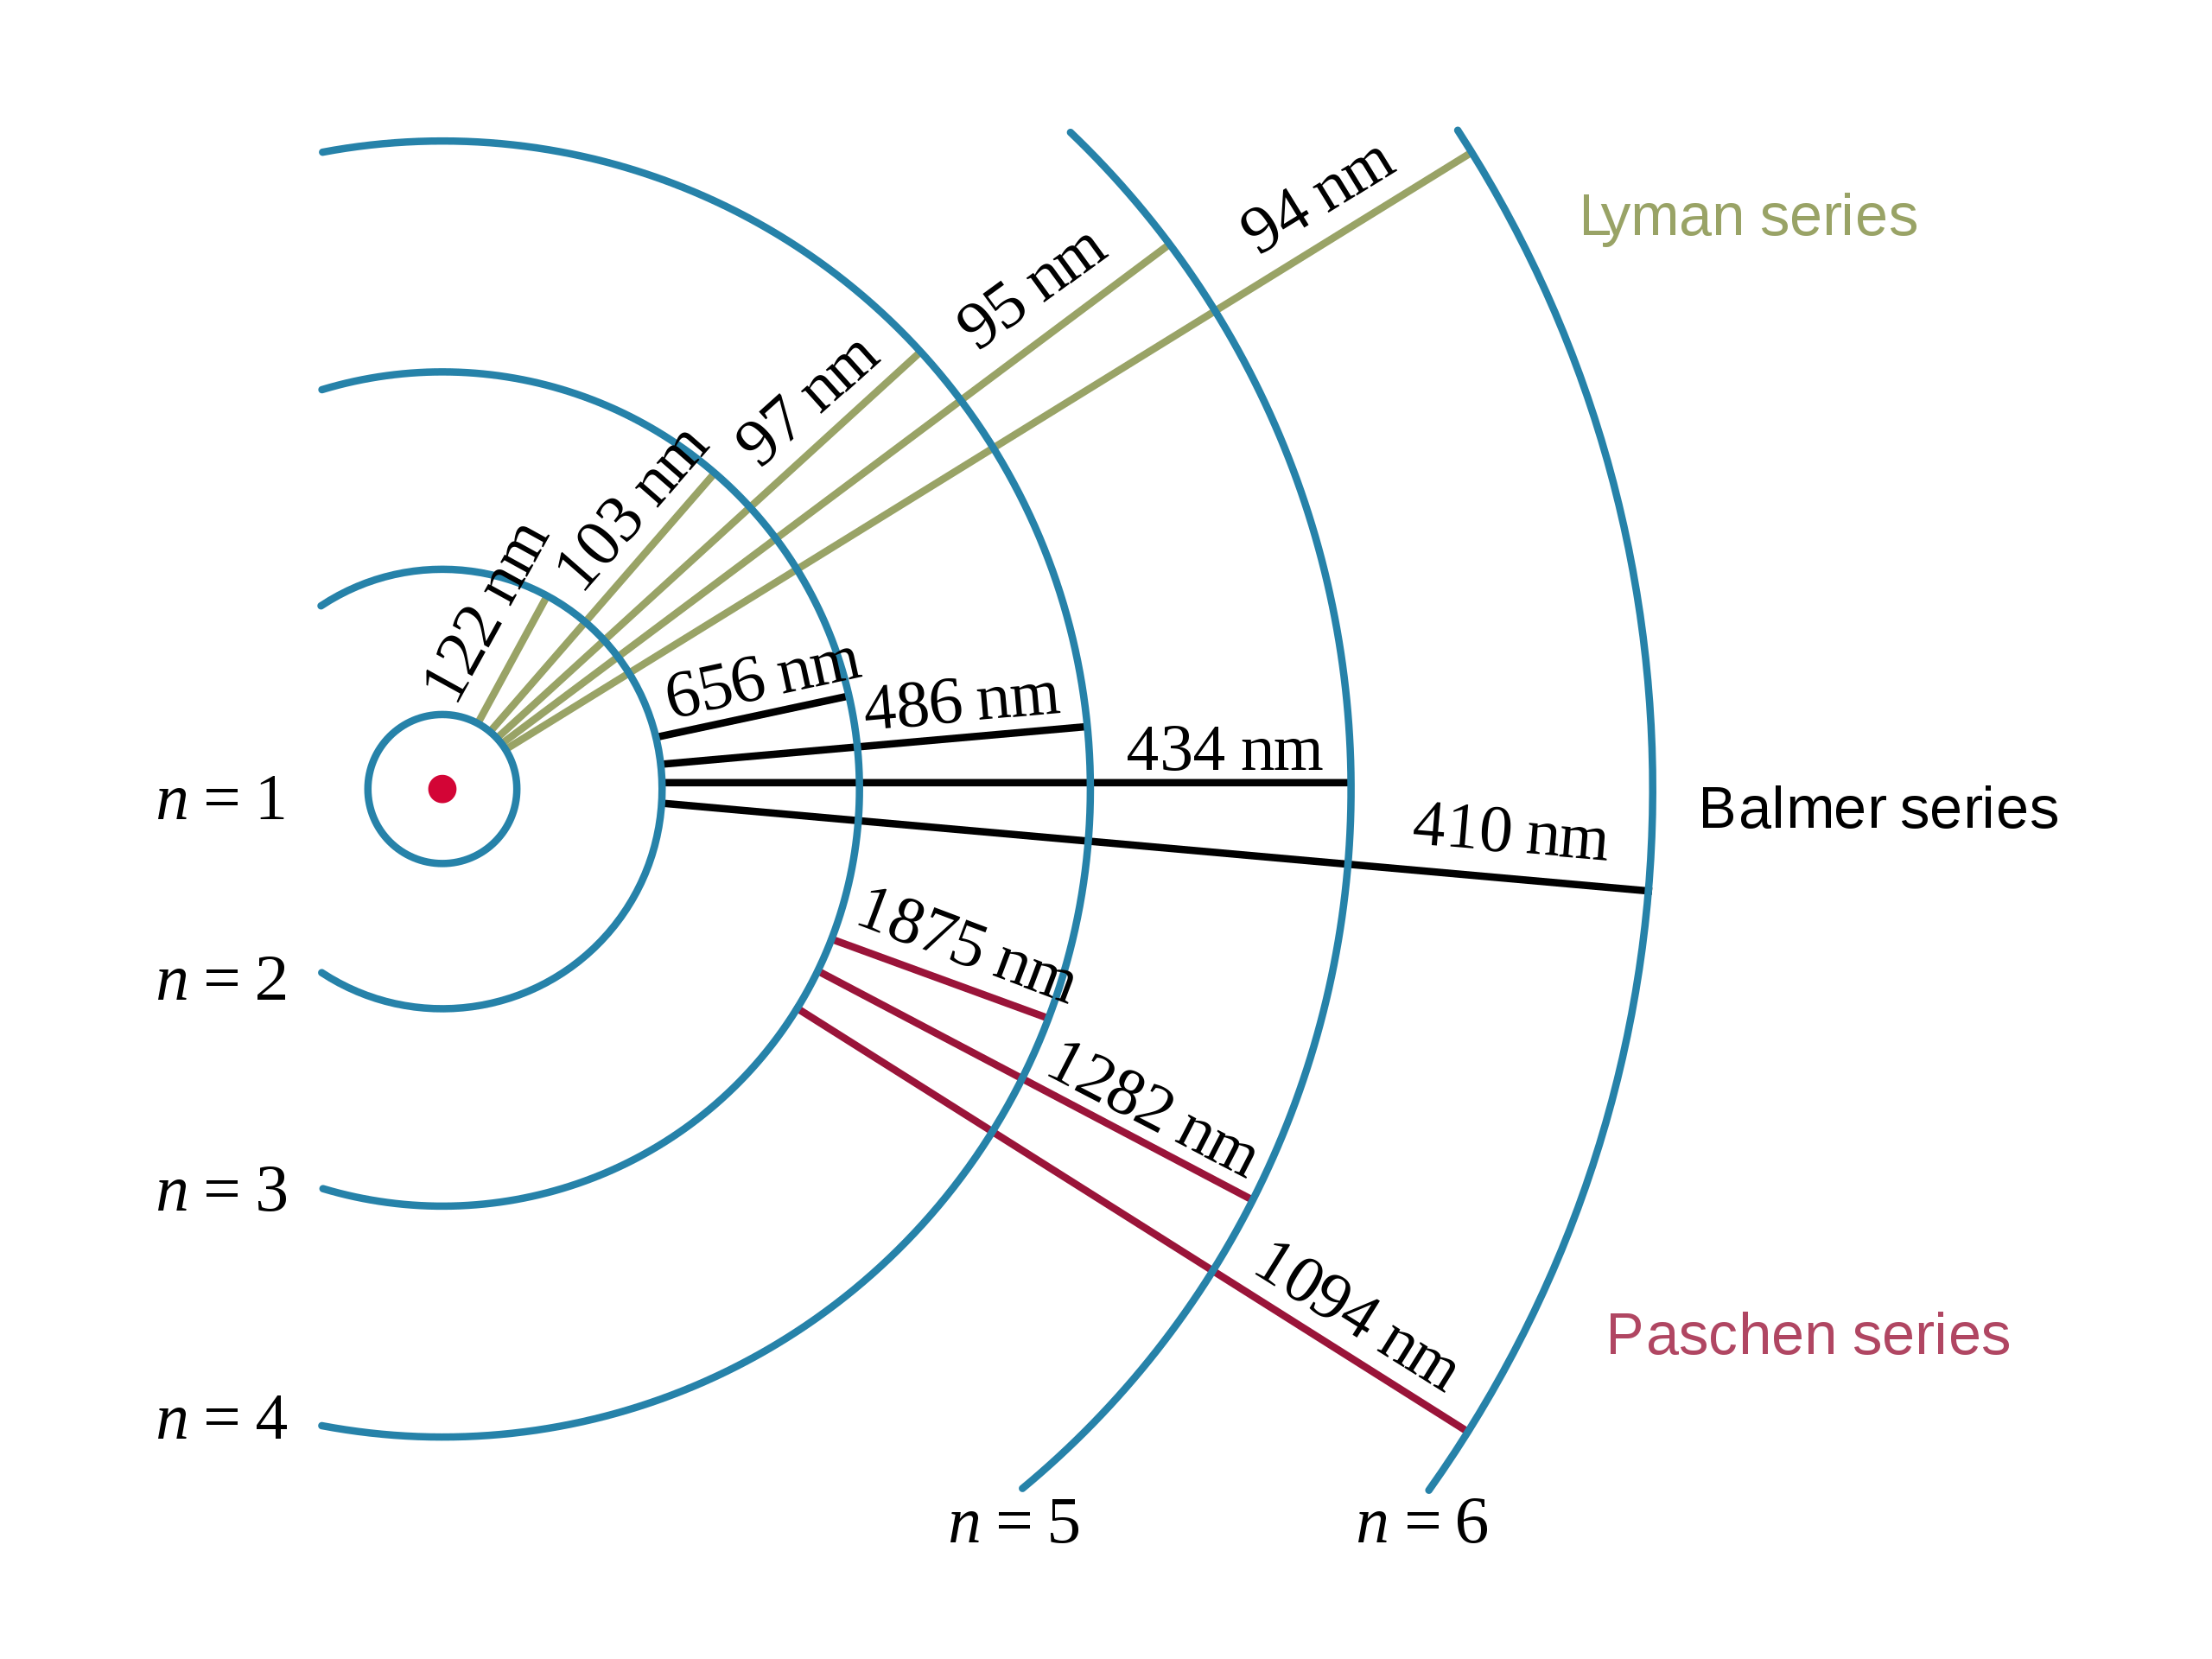
\includegraphics[scale=0.07]{h_spectra}
  \end{center}
\end{frame}

\begin{frame}{Practice: Using the Rydberg Equation}
  Use the Rydberg formula to predict which electronic transition in
  a hydrogen atom has the longest wave length: from $n = 2$ to $n = 1$,
  from $n = 3$ to $n = 2$, or form $n = 4$ to $n = 3$.
  \begin{center}
    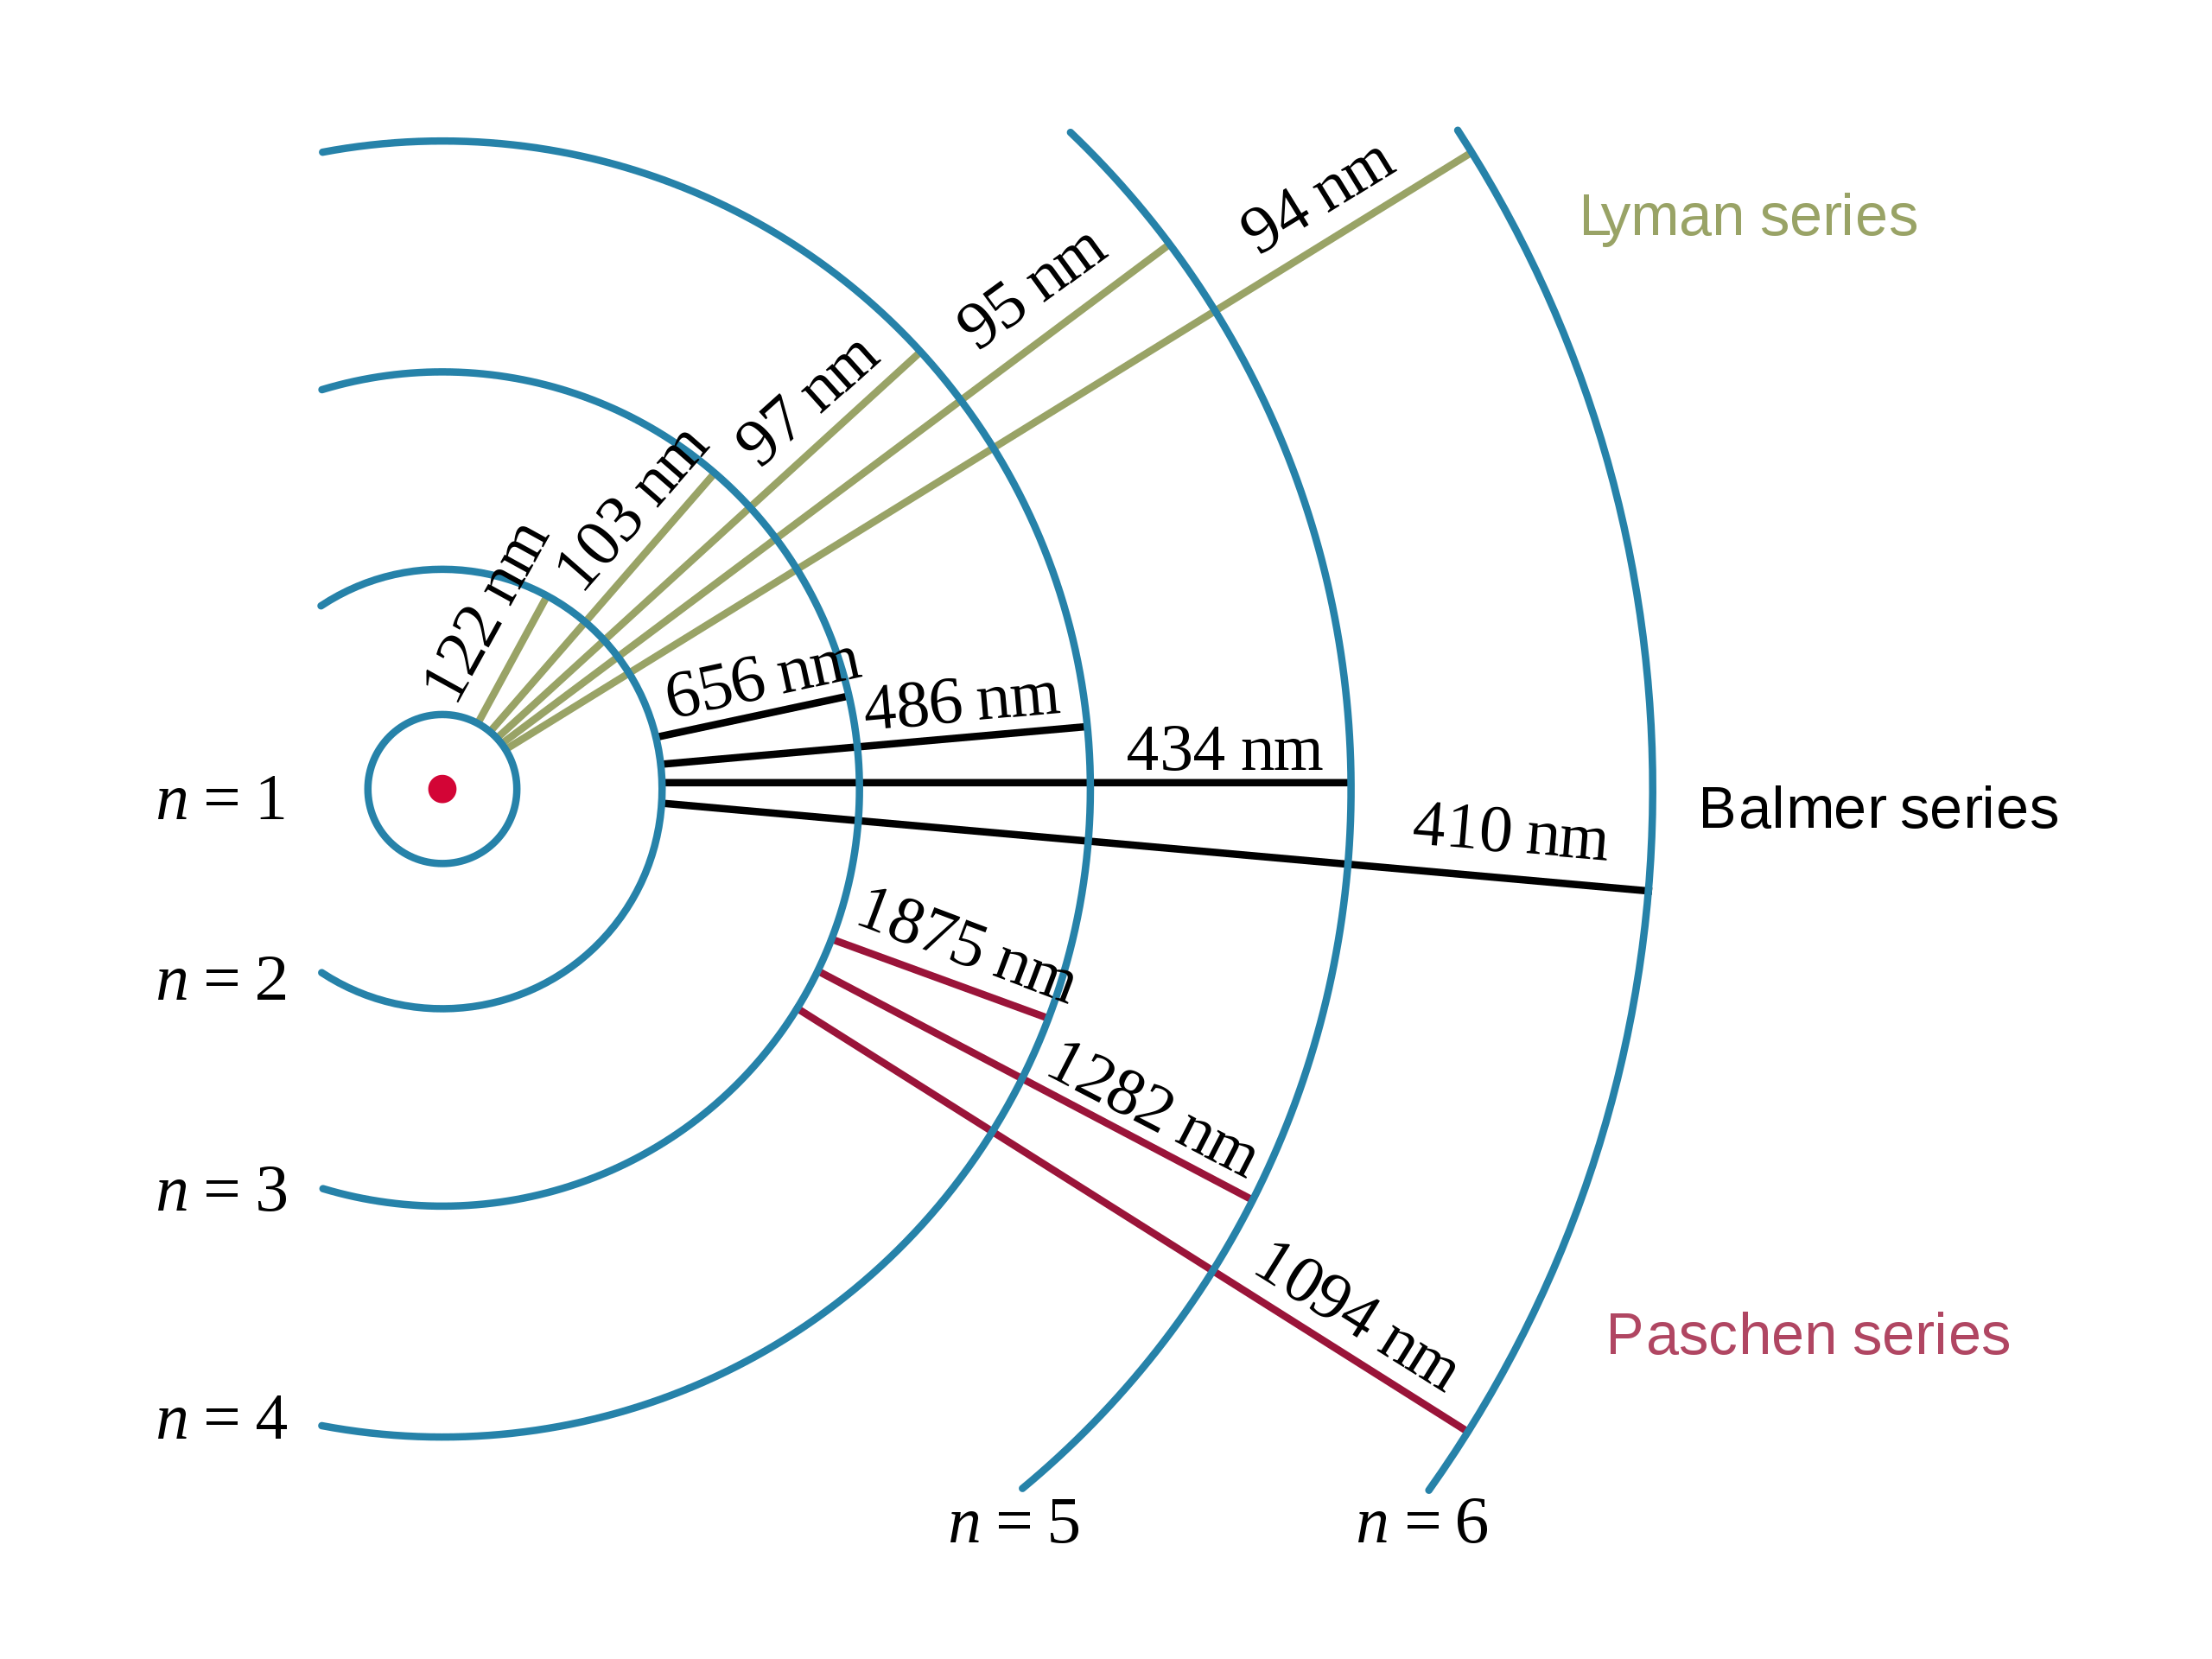
\includegraphics[scale=0.08]{h_spectra}
  \end{center}  
\end{frame}

\end{document}
